\documentclass{article}
\usepackage{graphicx} % Required for inserting images
\usepackage{multirow,booktabs}
\usepackage[table]{xcolor}
\usepackage[margin=.5in]{geometry}
\usepackage{amsmath}
\usepackage{amssymb}
\usepackage{amsfonts}
\usepackage{empheq}
\usepackage{hyperref}
\usepackage{blindtext}
\hypersetup{
    colorlinks=true,
    linkcolor=blue,
    filecolor=magenta,      
    urlcolor=cyan,% Requires: \usepackage{amsmath}
    pdftitle={Gravitation Notes},
    pdfauthor={Rudresh D. Gade}
    pdfpagemode=FullScreen,
    }


\graphicspath{ {./images/} }

\newenvironment{proof}{\paragraph{Proof:}}{\hfill$\square$}
\newenvironment{solution}{\paragraph{Solution:}}{\hfill$\square$}
\newenvironment{exercise}{\paragraph{Exercise:}}

\newtheorem{theorem}{Theorem}[section]
\newtheorem{defn}{Definition}[section]
\newcommand\note[1]{\textcolor{blue}{#1}}
\title{Gravitation Notes}
\author{Rudresh D. Gade}
\date{\today}

\begin{document}
\maketitle
\tableofcontents

\newpage

\section{Introduction}
\subsection{Why we need to replace the Newtonian Gravity. }
This course is about the modern theory of gravity-general relativity(GR).
\\



In Newton's theory, two point masses attract each other with a gravitational force of magnitude.


$$F = \frac{Gm_1m_2}{r_{12}^2}$$


where


$$G = 6.67 \times 10^{-11} \, \mathrm{Nm^2/kg^2}$$


and $r_{12}$ is the distance between them. Newtonian force acts instantaneously. The force on one mass depends on the position of the other mass at the same time! This is inconsistent with special relativity, where no signal can travel faster than the speed of light. So Newton's theory can at best be an approximation to a more `complete theory' in a regime where special relativistic effects are negligible.
\\
Consider the scenario where we have a mass $M$ large enough for gravity to be important. Consider a `test particle', with mass $m \ll M$ at a radius $R$ away from $M$. The escape velocity for small mass is $v$,


$$v^2 = \frac{2GM}{R}.$$ If $M$ is very large, we can have $v > c$, which is not possible in special relativity (SR).


Define $$\frac{2GM}{c^2} = R_S$$ Then $$\frac{v^2}{c^2} = \frac{R_S}{R}$$ and $R_S$ depend, apart from some fundamental constants, only on the mass $M$.


\note{Consider a star of radius $R$ and mass $M$. We can compute $\frac{R_S}{R}$ for the star. If that is greater than 1, or even close to 1, it means that we cannot neglect SR effects.} 
Plenty of astrophysical objects for which both gravity and relativity are important. We need a new theory of gravity in this regime. This theory is GR.
\\ \\ \\
The theory of General Relativity (GR) is not sufficient to describe all gravitational phenomena. In particular, when the radius of a star approaches the Schwarzschild radius ($R_S$), GR needs to be combined with Special Relativity (SR). However, even GR+SR is not enough when the radius of the star approaches Planck length ($l_\text{Planck}$), which is a regime in which gravity, quantum mechanics, and SR are all important. In this regime, a new theory of ``Quantum Gravity'' is needed, but it remains an unsolved problem. Therefore, \textbf{GR is at best an approximate theory}.

\subsection{Newtonian Gravity}
Let us take a closer look at the Newtonian gravity law:


$$\mathbf{F}_G = -\frac{G M m}{|\mathbf{r}_{12}|^2} \hat{\mathbf{r}}_{12}$$


We can write $\mathbf{F}_G = -m \nabla \Phi$ and


$$\Phi(\mathbf{x}) = -\frac{G M}{|\mathbf{r}_{12}|}$$


If there are many large masses $M_A$, the gravitational potential at $\mathbf{x}$


$$\Phi(\mathbf{x}) = -\sum_A \frac{G M_A}{|\mathbf{x} - \mathbf{x}_A|}$$


where $\mathbf{x}_A$ is the position vector of $M_A$.


If there is a continuous distribution of mass density $\rho(\mathbf{x}_0)$,


$$\Phi(\mathbf{x}) = -\int \frac{G \rho(\mathbf{x}_0)}{|\mathbf{x} - \mathbf{x}_0|} d^3 x_0$$


Define the Newtonian gravitational field $\mathbf{g} = -\nabla \Phi$. We then have the \textbf{Gauss law for gravity}:


$$\nabla \cdot \mathbf{g} = -4\pi G \rho(\mathbf{x})$$



\begin{exercise}
Show that the Gauss law for gravity follows from the expression for $\Phi$.    
\end{exercise}

\begin{solution}
\begin{align*}
\nabla \cdot \mathbf{g} &= \nabla \cdot (-\nabla \Phi) \\
&= -\nabla^2 \Phi \\
&= -\nabla^2 \left( -\int \frac{G \rho(\mathbf{x}_0)}{|\mathbf{x} - \mathbf{x}_0|} d^3 x_0 \right) \\
&= -\int G \rho(\mathbf{x}_0) \nabla^2 \left( \frac{1}{|\mathbf{x} - \mathbf{x}_0|} \right) d^3 x_0 \\
&= -\int G \rho(\mathbf{x}_0) \cdot 4\pi \delta(\mathbf{x} - \mathbf{x}_0) d^3 x_0 \\
&= -4\pi G \rho(\mathbf{x})
    \end{align*}    
\end{solution}



\begin{exercise}
When $\rho$ is spherically symmetric, integrate both sides of Gauss law over the volume inside a sphere of radius $r$ containing the mass entirely and show that $\Phi = -\frac{GM}{r}$ where $\int \rho(\mathbf{x}_0) d^3 x_0 = M$.    
\end{exercise}



\begin{solution}
\begin{align*}
\int \nabla \cdot \mathbf{g} d^3 x &= \int -4\pi G \rho(\mathbf{x}) d^3 x \\
\int \nabla \cdot \mathbf{g} d^3 x &= -4\pi G M \\
\oint \mathbf{g} \cdot d\mathbf{S} &= -4\pi G M \\
g \cdot 4\pi r^2 &= -4\pi G M \\
g &= -\frac{GM}{r^2} \\
\Phi &= -\int g dr = -\int \left( -\frac{GM}{r^2} \right) dr = -\frac{GM}{r}
\end{align*}    
\end{solution}
\\
Newton's law of gravitation, which describes the gravitational force $\mathbf{F}$, is given by:


$$\mathbf{F} = -m_g \nabla \Phi$$


where $m_g$ is the gravitational mass and $\Phi$ is the gravitational potential.


Newton's second law, which relates the force $\mathbf{F}$ to the acceleration $\mathbf{a}$, is given by:


$$\mathbf{F} = m_I \mathbf{a}$$


where $m_I$ is the inertial mass.


Equating the two, we get:


$$m_I \mathbf{a} = -m_g \nabla \Phi$$


Since the gravitational mass $m_g$ is equal to the inertial mass $m_I$, we can simplify to get:


$$\mathbf{a} = -\nabla \Phi$$


This shows that the acceleration of an object under gravity is determined by the gradient of the gravitational potential.

\subsection{To be in rest or not to be in rest?}
In an inertial frame, the acceleration of an object under gravity is given by:


$$\frac{d^2\mathbf{x}}{dt^2} = -\nabla\Phi = \mathbf{g}(\mathbf{x},t)$$


Now, let's consider a non-inertial frame $\tilde{\mathbf{x}} = \mathbf{x} - \mathbf{b}(t)$. The acceleration in this frame is:


$$\frac{d^2\tilde{\mathbf{x}}}{dt^2} = \tilde{\mathbf{g}} = \mathbf{g}(\mathbf{x},t) - \frac{d^2\mathbf{b}}{dt^2}$$


If $\mathbf{g}$ is independent of $\mathbf{x}$ (i.e., a uniform gravitational field), we can choose $\mathbf{b}$ such that:


$$\frac{d^2\tilde{\mathbf{x}}}{dt^2} = \tilde{\mathbf{g}} = 0$$


in the new non-inertial frame.


This means that in the new accelerating frame of reference, the test particle is at rest or in uniform motion.


\textbf{Conclusion:} \note{It is not possible to distinguish between an object falling freely under a uniform gravitational field and an object at rest in an accelerated frame of reference.}
\subsection{Equivalence Principle}
This observation leads to the following Equivalence principles:


\textbf{Weak Equivalence Principle:} The motion of freely falling particles is the same in a gravitational field and a uniformly accelerated frame in small enough regions of spacetime where the gravitational field can be assumed uniform.


\textbf{Einstein Equivalence Principle:} In small enough regions of spacetime, the laws of physics reduce to those of special relativity - it is impossible to detect a gravitational field by means of local experiments.


\note{`Local experiments' are \textbf{ANY} ones, not just those involving freely falling particles.
}
\subsection{Newtonian Gravity in non uniform gravitational field}
What happens in Newtonian gravity when the gravitational field $\mathbf{g}$ is not uniform? Consider two test particles close by at $\mathbf{x}$ and $\mathbf{x} + \mathbf{N}$.


$$\frac{d^2\mathbf{x}}{dt^2} = \mathbf{g}(\mathbf{x},t)$$

$$\frac{d^2(\mathbf{x} + \mathbf{N})}{dt^2} = \mathbf{g}(\mathbf{x} + \mathbf{N},t)$$


Subtracting the two equations, we get:


$$\frac{d^2\mathbf{N}}{dt^2} = \mathbf{g}(\mathbf{x} + \mathbf{N},t) - \mathbf{g}(\mathbf{x},t) = (\mathbf{N} \cdot \nabla)\mathbf{g} + O(N^2)$$


by Taylor expanding $\mathbf{g}(\mathbf{x} + \mathbf{N},t)$ about $\mathbf{x}$.


In components,


$$\frac{d^2N_i}{dt^2} = \sum_{j=1}^3 N_j \frac{\partial g_i}{\partial x_j}$$


Now, $g_i = -\frac{\partial \Phi}{\partial x_i}$. So


$$\frac{d^2N_i}{dt^2} + \sum_{j=1}^3 E_{ij} N_j = 0$$


where $E_{ij} = -\frac{\partial g_i}{\partial x_j} = \frac{\partial^2 \Phi}{\partial x_i \partial x_j}$. This equation is called the \textbf{Newtonian geodesic deviation equation}. Note: $E_{ij} = E_{ji}$.


Gauss' law for gravity was $\nabla^2 \Phi = 4\pi G \rho$. So the structure of Newtonian gravity is:
\begin{enumerate}
    \item $\frac{d^2N_i}{dt^2} + \sum_{j=1}^3 E_{ij} N_j = 0 \quad \text{(Geodesic deviation)}$
    \item $E_{ij} = E_{ji}$
    \item $\nabla^2 \Phi = 4\pi G \rho \quad \text{(Field equation)}$
    \item $\frac{\partial E_{ij}}{\partial x_k} - \frac{\partial E_{kj}}{\partial x_i} = 0 \quad \text{(Show this)}$
\end{enumerate}
\newpage
\begin{exercise}
    $\frac{\partial E_{ij}}{\partial x_k} - \frac{\partial E_{kj}}{\partial x_k} = 0 \quad $
\end{exercise}

\begin{solution}
    To show that $\frac{\partial E_{ij}}{\partial x_k} - \frac{\partial E_{kj}}{\partial x_i} = 0$, we can start by using the definition of $E_{ij}$:


$$E_{ij} = \frac{\partial^2 \Phi}{\partial x_i \partial x_j}$$


Now, let's compute the two terms:


$$\frac{\partial E_{ij}}{\partial x_k} = \frac{\partial}{\partial x_k} \left( \frac{\partial^2 \Phi}{\partial x_i \partial x_j} \right) = \frac{\partial^3 \Phi}{\partial x_k \partial x_i \partial x_j}$$


$$\frac{\partial E_{kj}}{\partial x_i} = \frac{\partial}{\partial x_i} \left( \frac{\partial^2 \Phi}{\partial x_k \partial x_j} \right) = \frac{\partial^3 \Phi}{\partial x_i \partial x_k \partial x_j}$$


Since the order of partial derivatives is interchangeable, we have:


$$\frac{\partial^3 \Phi}{\partial x_k \partial x_i \partial x_j} = \frac{\partial^3 \Phi}{\partial x_i \partial x_k \partial x_j}$$


Therefore,


$$\frac{\partial E_{ij}}{\partial x_k} - \frac{\partial E_{kj}}{\partial x_i} = \frac{\partial^3 \Phi}{\partial x_k \partial x_i \partial x_j} - \frac{\partial^3 \Phi}{\partial x_i \partial x_k \partial x_j} = 0$$

\end{solution}

\section{Special Relativity }
\subsection{Sacred Medium}
Velocities of O and O' frame are not the same 
    \begin{align*}
        V^{x'} = V^{x} -v \\
        V^{y'} = V^y \\
        V^{z'} = V^z 
    \end{align*}
 
People surmised the existence of medium called ether with a special frame of reference in which light travels at speed c.

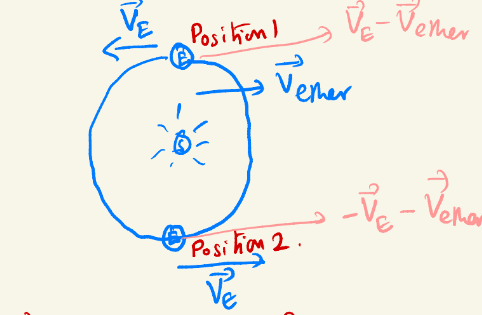
\includegraphics[width=0.5\linewidth]{ether.png}\\ \\
   $\vec{V_E}$ = vel. w.r.t. Sun
   \\
   $\vec{V_{ether}}$= vel. of ether w.r.t sun
   \\
   Vel. of light at position 1 = $c-\vec{V_E}+\vec{V_{ether}}$\\
   Vel. of light at position 2 = $c+\vec{V_E}+\vec{V_{ether}}$


Difference in two velocities = $2\vec{V_{ether}}$
\\ \\ But Michelson Morley experiment did not observe any change in the velocity \\
$\implies $nonexistence of ether.

\subsection{Spacetime}
\textbf{Time is not a parameter unlike in Newtonian Mechanics.}
\\
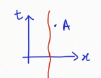
\includegraphics{worldline.png}
\\
A particle describes a tragectory in spacetime called a "\textbf{World line}". The red line in the spacetime diagram is a world line.
\\
The central assumption of secial relativity(SR):\\
\begin{itemize}
    \item Light travels with speed c in all inertial frames.
    \item Using this, i can deduce that there is an \textbf{invariant interval} in spacetime.
\end{itemize}
This interval is $$ds^2=-c^2dt^2+dx^2+dy^2+dz^2$$
For all inertial frames, this interval is invariant.
It is called\textbf{ Minkowski Line Element}. we can write it in matrix notation:\\
$$ds^2=(cdt,dx,dy,dz)\begin{pmatrix}
    -1&0&0&0\\
    0&1&0&0\\
    0&0&1&0\\
    0&0&0&1
\end{pmatrix} \begin{pmatrix}
    cdt\\dx\\
    dy\\
    dz
\end{pmatrix}$$
$$ds^2=d\Bar{x}^T \eta d\Bar{x}$$
where $d\Bar{x}= \begin{pmatrix}
    cdt\\dx\\dy\\dz
\end{pmatrix}$ and $\eta =\begin{pmatrix}
    -1&0&0&0\\
    0&1&0&0\\
    0&0&1&0\\
    0&0&0&1
\end{pmatrix} $
\\ \\ 
$\eta $ is called \textbf{'Minkowski Matrix'} of Minkowski Spacetime.\\
\\
The distance squared between 2 points in this space is defined as $$\Delta s^2=-c^2(\Delta t)^2+(\Delta x)^2+(\Delta y)^2+(\Delta z)^2$$
\\
The 2 points are:
\begin{itemize}
    \item Spacelike seperated if $(\Delta s)^2>0$
    \item Timelike seperated if $(\Delta s)^2<0$
    \item Null seperated if $(\Delta s)^2=0$
\end{itemize}
\note{If 2 points are null seperated,$\implies ( ds)^2=0 \implies (\frac{dx}{dt})^2+(\frac{dy}{dt})^2+(\frac{dz}{dt})^2=c^2$\\ Therefore the locus of points null seperated from point P is called its '\textbf{light cone}' }

 Timelike worldlines always lie inside the lightcone at every point on the world line. This is a consequence of speed being $<c.$ \\
Points that are spacelike seperated lie outside of each other lightcone.\\
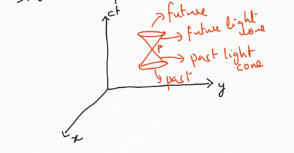
\includegraphics[width=0.5\linewidth]{causal structure.png} \\
This is called the \textbf{Casual Structure} of SR.
\subsection{Lorentz Transformation}
Take 2 inertial frames O and O', O' is moving in x- direction  with speed v.\\
We want transformations (x,t) $\xrightarrow{}$ (x',t') such that $$ds^2=-c^2dt'^2+dx'^2=-c^2dt^2+dx^2$$
In Matrix Form:
$$\Bar{X'}=\Lambda \Bar{X}$$
$$\begin{pmatrix}
    ct'\\x'\\y'\\z'
\end{pmatrix}=\begin{pmatrix}
    \gamma &-\beta \gamma&0&0\\-\beta \gamma &\gamma &0&0\\0&0&1&0\\0&0&0&1
\end{pmatrix}\begin{pmatrix}
    ct\\x\\y\\z
\end{pmatrix}$$ where $\beta = \frac{v}{c}$
\\ \\ \\
\textbf{Velocity Transformation}:\\
O measures $(x(t),y(t),z(t))$\\
O' measures $(x'(t'),y'(t'),z'(t'))$
$$V^{x'} = \frac{dx'}{dt'}=\frac{\gamma(dx-vdt)}{\gamma(dt-\frac{v}{c^2}dx)}= \frac{V^{x}-v}{1-\frac{v}{c^2}V^{x}}$$
$$V^{y'} = \frac{dy'}{dt'}=\frac{V^{y}\sqrt{1-\frac{v^2}{c^2}}}{1-\frac{v}{c^2}V^{x}}$$
$$V^{z'} = \frac{dz'}{dt'}=\frac{V^{z}\sqrt{1-\frac{v^2}{c^2}}}{1-\frac{v}{c^2}V^{x}}$$

This reduces to Newtonian Mechanics if $v<<c$.
\\ \\ \\
\textbf{Let} $$\mathbf{V^x=c \implies V^{x'}= c}$$
\note{    Thus The speed of Light is Invariant in Spacetime
}
\\
Recall That the Minkowski line element is invariant under thes transformations.
$$ds^2= d\Bar{x}^T \eta d\Bar{x}= d\Bar{x'}^T \eta d\Bar{x'} $$
But $$\Bar{X'}=\Lambda \Bar{X}$$
$$ds^2= d\Bar{x}^T \eta d\Bar{x}= d\Bar{x'}^T \Lambda^T \eta \Lambda d\Bar{x'}$$
\begin{equation}
\implies \eta =\Lambda^T \eta \Lambda   
\end{equation}
This is sometimes taken as the definition for lorentz matrices.The Matrices satisfying (4) forms a group "\textbf{Lorentz Group}"
\\ \\
\\
Define Proper Time $\tau$ as
$$ds^2=-c^2d\tau^2$$ it is the time on a clock attached to the particle. it is invariant under the lorentz transformations.
\subsection{Special Relativistic Mechanics}
4- Vectors : Directed line segments in 4D spacetime.
$$\Bar{a}= a^t\hat{e_t}+a^x\hat{e_x}+a^y\hat{e_y}+a^z\hat{e_z} = \sum_\alpha a^\alpha \hat{e_\alpha} $$
\newpage
Thus $$\Bar{a}\cdot \Bar{b}:=a^\alpha \hat{e_\alpha} \cdot a^\beta \hat{e_\beta}= a^\alpha b^\beta \eta_{\alpha\beta}$$
Consider the position vector in spacetime: $$\Bar{x}= x^\alpha\hat{e_\alpha}$$
$$\Bar{x}\cdot \Bar{x}= a^\alpha\eta_{\alpha\beta} b^\beta $$
Now consider a lorentz traansformation from frame O to O':$$\Bar{X'}=\Lambda \Bar{X}$$
$$\Bar{x'}\cdot \Bar{x'}= (\Lambda \Bar{x})^T \eta (\Lambda \Bar{x})$$
$$= \Bar{x}^T \Lambda^T \eta \Lambda \Bar{x} $$
$$=\Bar{x}^T \eta \Bar{x}$$
Thus the normed squared of the position vector in spacetime is invariant under lorentz transformation.
\\ \\ \\
\textbf{4-Velocity}:
Define $\mathbf{\Bar{u}= \frac{d\Bar{x}}{d\tau}}$ to be the 4-velocity of a massive particle where $\tau$ is the proper time and $\Bar{x}$ is the position vector. \\
4-velocity is the tangent to the worldline at every point.\\
\note{4-velocity is only for \textbf{timelike} worldline so far. }
\\ \\ \\
\textbf{Relation between }$\mathbf{\tau}$ \textbf{and t}:
$$ds^2= -c^2\tau^2= -c^2dt^2+dx^2+dy^2+dz^2 $$
$$c^2\tau^2= c^2dt^2(1-\{\frac{dx}{dt})^2+(\frac{dy}{dt})^2+(\frac{dz}{dt})^2\})$$
$$=c^2dt^2(1-\frac{v^2}{c^2})$$
$$d\tau=dt\sqrt{1-\frac{v^2}{c^2}}$$

\textbf{The components of} $\Bar{u}$:

$$u^\alpha=\frac{dx^\alpha}{d\tau}$$
$$u^t=\frac{cdt}{d\tau}=c\gamma$$
$$u^{x,y,z}=\frac{d\{x,y,z\}}{d\tau}= \frac{d\{x,y,z\}}{dt}\cdot \frac{dt}{d\tau}= V^{\{x,y,z\}}\gamma$$
$$\Bar{u}=(c\gamma,\gamma\Bar{V})$$
\begin{exercise}
    Using dot product of 4-vectors, show that $$\Bar{u}\cdot \Bar{u}= -c^2$$
\end{exercise}
\begin{solution}
    $$\Bar{u}\cdot \Bar{u}= u^\alpha \eta u^\beta$$
    $$\Bar{u}\cdot \Bar{u}= \gamma^2(-c^2+v^2)$$
    $$\Bar{u}\cdot \Bar{u}= \frac{-c^2(c^2-v^2)}{c^2-v^2}=-c^2$$
\end{solution}

\vspace{4mm}
\textbf{4-acceleration}:=$$\Bar{a}= \frac{d\Bar{u}}{d\tau}$$\\
\textbf{4-momentum}:= $$\Bar{p}=m\Bar{u}=(mc\gamma,m\gamma\Bar{v})$$\\ \\
\hspace{4mm}
\\

For small speeds $v<<c$:
$$p^t= mc\gamma= mc\frac{1}{\sqrt{1-\frac{v^2}{c^2}}}$$
$$\approx mc(1+\frac{v^2}{2c^2} + \cdots )$$
$p^t= \frac{E}{c} $ where $E = mc^2(1+\frac{v^2}{2c^2} + \cdots )$
$$\Vec{p}= m\gamma\Vec{v}= \frac{m\Bar{v}}{\sqrt{1-\frac{v^2}{c^2}}}=m\Vec{v}(1+\frac{v^2}{2c^2}+\cdots)$$

$$\Bar{p}=(\frac{E}{c},\Vec{p})$$
Now $$\Bar{p}\cdot \Bar{p}= -m^2c^2$$
$$\implies E = \sqrt{m^2c^4 + |\vec{p}|^2c^2}$$
$$|\frac{\vec{v}}{c}|= \frac{|\vec{p}|}{\frac{E}{c}}$$
As $m\xrightarrow{}0$, $$E^2 = p^2c^2= |\vec{p}|^2\implies |\vec{v}|=c$$
So massless particles move with speed of light.

\note{light follows a 'straight' path in a curved spacetime!! .\\ }

\textbf{Gravity is the \textbf{intrinsic} property of the curved spacetime and light follows the straight line  
in this curved spacetime} 

\section{Topology }

\begin{defn}
    A set T with a collection of subsets of X is a topology if:
    \begin{enumerate}
        \item Trivial set X and empty set is in T.
        \item if A and B are in T, then $A\bigcap B \in T$
        \item whenever two or more subsets are in T, So is thier arbitiary union.
        \ 
    \end{enumerate}
\end{defn}
The Set + Topology on a set = \textbf{Topological Set} 
\subsection{Open set}
A set in T is called an \textbf{Open Set}.

\subsection{Continuous Function }
If $f$ is a function $f:X \mapsto Y$ where X,Y are topological spaces.Then $f$ is \textbf{continuous} at a point x$\in$ X iff for  any neighbourhood V of $f(x)$ in Y $\exists$ a neighbourhood U of X such that $F(U) \subseteq V$.  

\subsection{Homeomorphism}
A function $f:X \mapsto Y$ where X,Y are topological spaces.Then $f$ is a homeomorphism if:
\begin{enumerate}
    \item $f(x)$ is one-one and onto 
    \item $f(x)$ is continuous 
    \item $f^{-1}(x)$ is continuous
\end{enumerate}


\subsection{Topological Manifold}
\begin{defn}[Basis of Topology]
    Collection of subsets of X,B s.t. every $x\in X$ lies in some element B and if $x \in B_1 \bigcap B_2$, there is a third element $B_3 \subset B_1 \bigcap B_2$ containing x. 
\end{defn}
\begin{defn}[Second countability]
    It has a countable basis for its topology. 
\end{defn}
\begin{defn}
    A Topological space is called Topological manifold if it has following properties:
    \begin{enumerate}
        \item Housdorffness (any 2 points have disjoint nbds)
        \item Paracompactness ( It is second countable(Lindleof property))
        \item Locally Euclidean(Every point in X has a nbd. homeomorphic to $R^n$)
    \end{enumerate}
        
\end{defn}

\begin{defn}[Transition Function or chart]
    The map $\varPhi : X\mapsto R_n $ is called a transition function if it is smooth.

\end{defn}

\begin{defn}[Atlas]
    A $C^{\infty}$ Atlas is a collection of sets $U_{\alpha}$ along with $\varPhi_{\alpha} $ such that ($U_\alpha,\varphi_\alpha$) is a smoothly compatible chart.
\end{defn}
\begin{defn}
The collection of all smoothly compatible charts is called \textbf{MAXIMAL ATLAS} for X. 

\end{defn} 

\begin{theorem}[Whitney Theorem]
    A smooth manifold is always embedded in a higher dimensional euclidean space.
    
\end{theorem}

 A topological manifold with maximal smooth atlas is called \textbf{smooth manifold}.
\\
The Physics Laws should be independent of the general coordinates.
\section{Differential geometry}
\subsection{Vectors}
\begin{defn}
    A \textbf{Vector} at a point p in a smooth manifold is a linear map $X: C^{\infty} \mapsto \mathbb{R}$ which satisfies the following rule:$$X(fg)=X(f)g +fX(g)  \forall f,g \in C^{\infty}$$ It is also called a \textbf{derivation}.
\end{defn}
The set of all derivation at the point p forms a vector space $T_p M$ called the \textbf{Tangent space} at p .
\\
The vector can also be thought of as a derivative. Hence $$V = \sum_{\mu} V^{\mu} \frac{\partial}{\partial x^{\mu}}   $$ Here the $\{\frac{\partial}{\partial x{\mu}} \}$ forms a basis for the tangent space.We introduce the Einstein Summation as $$V = \sum_{\mu} V^{\mu} \frac{\partial}{\partial x^{\mu}} = V^i\frac{\partial}{\partial x^{i}}$$  Thus $$V(f) = V^i\frac{\partial}{\partial x_{i}} (f)$$
\\
If the map $F : M \mapsto \mathbb{R}$ is a diffeomorphism then the map $F^* : T_p M \mapsto T_{F(p)} N$ is an isomorphism between the two tangent spaces $T_pM , T_{F(p)} N$ 

\subsubsection{Change of Basis}
Let $x^i$ and $x^{x'}$ be two coordinate systems of the same manifold. A vector V is invariant under the transformation. Thus $$V = V^i \frac{\partial}{\partial x^{i}} = V^{j'} \frac{\partial}{\partial x^{j'}} $$
$$V^i \frac{\partial x^{j'}}{\partial x^{i}} \frac{\partial}{\partial x^{j'}} = V^{j'} \frac{\partial}{\partial x^{j'}} $$ 
\begin{center}
\boxed{$$V^i \frac{\partial x^{j'}}{\partial x^{i}}  = V^{j'} $$}
\end{center}
Thus the vector tranform by the above rule under a coordinate transformation.
\subsection{Covector}
\begin{defn}[Dual vector space]
    A dual vector space $V^*$ of V is the collection of all bounded linear map $F : V \mapsto \mathbb{R} $.

\end{defn}
\textbf{Covectors} are the elements of the $V^*$.
\\ \\
The Covectors also form a vector space $T^*_p M$. 
Label the basis of the dual vector space of V as $\{ dx^i \}$

Let $V = T_pM,V^* = T^*_pM$ and let the basis of V and $V^*$ be $\{\frac{\partial}{\partial x^i}\},\{ dx^i \}$
 \\
Then we have the following rule:
$$\boxed{dx^i (\frac{\partial}{\partial x^j}) = \delta_j^i  }$$

if $w \in V^*$ Then $w = w_idx^i$ and $V = V^j \frac{\partial}{\partial x^j}$  

Thus $$w(V) = w_idx^i (V^j \frac{\partial}{\partial x^j})=w_i V^j dx^i ( \frac{\partial}{\partial x^j}) = w_i V^j \delta_j^i = w_i V^i = V(w)$$

Hence Vectors can be thought of acting on Covectors (Linear maps).

\subsubsection{Coordinate basis change }
\textbf{Postulate : }The Covectors are assumed to follow the following rule: 
$$\boxed{dx^{i'} =  \frac{\partial x^{i'}}{\partial x^i} dx^i}$$ 

\subsection{Tensor}
A natural extension of vectors and dual vectors is the concept of a \textbf{tensor}. Similar to how a dual vector is a linear map from vectors to $\mathbb{R}$, a tensor $T$ of type (or rank) $(k, l)$ is a multilinear map from a collection of dual vectors and vectors into $\mathbb{R}$:

\[
T: 
\underbrace{T_p^* \times \cdots \times T_p^*}_{k \text{ copies}} \times \underbrace{T_p \times \cdots \times T_p}_{l \text{ copies}} \to \mathbb{R} 
\]

Here, "$\times$" represents the Cartesian product, so $T_p \times T_p$ denotes the space of ordered pairs of vectors. The term "multilinear" indicates that the tensor behaves linearly in each of its arguments.
\\
In component notation we then write our arbitrary tensor as
\[
T = T^{\mu_1 \cdots \mu_k}_{\nu_1 \cdots \nu_l} \frac{\partial}{\partial x^{\mu_1}} \otimes \cdots \otimes \frac{\partial}{\partial x^{\mu_k}} \otimes dx^{\nu_1} \otimes \cdots \otimes dx^{\nu_l}
\]

The collection of all tensors of rank$(k,l)$ itself  forms a vector space. 
\subsubsection{Tensor Transformation}
Tensor follows the following transformation rule:
\[
T^{\mu'_1 \cdots \mu'_k}_{\nu'_1 \cdots \nu'_l} = \frac{\partial x^{\mu'_1}}{\partial x^{\mu_1}}  \cdots  \frac{\partial x^{\mu'_k} }{\partial x^{\mu_k}} \frac{\partial x^{\nu'_1}}{\partial x^{\nu_1}}  \cdots  \frac{\partial x^{\nu'_k} }{\partial x^{\nu_k}}  T^{\mu_1 \cdots \mu_k}_{\nu_1 \cdots \nu_l} 
\]

\subsection{Metric Tensor}
We want an analogue to the $"ds^2"$ in M. Define a symmetric rank$(0,2)$ Tensor A such that 
$$A = A_{ij} \frac{1}{2}[dx^i \otimes dx^j + dx^j \otimes dx^i ]$$
$$= A_{ij} dx^idx^j$$

Thus define $$dx^idx^j = \frac{1}{2}[dx^i \otimes dx^j + dx^j \otimes dx^i ]$$
Thus the special $rank (0,2)$ Tensor Feild that is symmetric is $$G = g_{ij}(x) dx^idx^j $$
G is called the \textbf{Metric Tensor}.\\ \\
We can define the inner (dot) product between two vectors at a point p from this mertic tensor as $$G_p(v,w) = \sum _{i,j} g_{ij} v^iw^j$$
$$= v^T g_p w$$ where $g_p-$ is the symmetric matrix of G

\note{if $g_p$ is symmetric and has positive eigenvalues then $$v^T g_p v = 0 \iff v=0$$                  }

square of the length of v is $G(v,v) = g_{i,j} v^iv^j$.\\
Comparing to $ds^2 = \eta_{ij} dx^idx^j$, we get that G is playing the role of $ ds^2$.
\\ \\
If G has all the eigenvalue to be positive then we say it to be \textbf{Reimannian Metric} and if it has 1 negetive and 3 positive eigenvalue the we call it \textbf{Lorentzian Metric}.
\subsubsection{Raising and Lowering of indices}
Consider the following Maps:\\
Covector $w:T_p M \mapsto \mathbb{R} $  \\
Vector    $V: T^*_p M \mapsto \mathbb{R}$ 
\\ Suppose we have a metric $G = g_{ij} dx^idx^j$ Then we have the inner (dot) product $\langle v_a,v_b \rangle_g = \sum g_{ij}v_a^iv_b^j$. 
\\
The operator $ \langle \cdot, v_b \rangle_g$ operates on a vector $v_a$ and gives a real number. Thus  $ \langle \cdot, v_b \rangle_g$ is a covector.
Now.
$$\langle v_a,v_b \rangle_g = \sum g_{ij}v_a^iv_b^j$$
$$\langle \cdot,v_b \rangle_g = \sum g_{ij}v_b^j$$
Thus $$(v_b)_i = \sum_j g_{ij} (v_b)^j $$
if $g$ is the matrix of G with components $g_{ij}$, Then $g_{-1} $ is the matrix formed by the components $g^{ij}$ \\
Define$$\boxed{G^{-1} = g^{ij} \frac{1}{2}[\frac{\partial }{\partial x^i} \otimes \frac{\partial}{\partial x^j} +\frac{\partial }{\partial x^j} \otimes \frac{\partial}{\partial x^i}   ]} $$  
Then $G^{-1}$ is an operator operating on covector giving a Real number. Thus it is a vector. \\ \\
Given a covector $(w_b)_j$. Then $g^{ij} (w_b)_j = w^i_b$  
In summary, $$g: T_pM \mapsto T^*_p M$$ $$g^{-1}: T^*_pM \mapsto T_p M$$  
Consider a $rank(1,2)$ Tensor $T(w_a,v_a,v_b)$ Then$$g_{il} T^i_{jk} = T_{ljk} \text{   and    }  g^{jl}T^i_{jk} = T^{il}_k$$
\\
For any Transformation from $rank(k,l)$ to $rank(a,b)$, $a+b=k+l$ always.
\\ \\ 
Now we know that $$G = g_{ij}dx^idx^j = \bar{dx}^T (g)\bar{dx}= ds^2$$
$eg.$ The Minkowski Metric : $ds^2 = \bar{dx}^T (\eta)\bar{dx}$ where $\eta =\begin{pmatrix}
    -1&0&0&0\\
    0&1&0&0\\
    0&0&1&0\\
    0&0&0&1
\end{pmatrix} $
\\
\note{g is a symmetric metric and the entries are in general functions.} 
\begin{theorem}[Spectral Theorem for symmetric matrices]
    Any symmetric matrix of real numbers can be diagonalised by an orthogonal matrix $Q$ where orthogonal matrix means $Q^{-1} = Q^T$
\end{theorem}

\subsubsection{Locally Minkowski }
$$ds^2 = \bar{dx}^T (g)\bar{dx}$$
Now do a coordinate transformation defined by the matrix $Q$ such that $x = Qx'$. Thus$$ds^2 = \bar{dx'}^T (Q^TgQ)\bar{dx'}$$ 
Choose $Q$ such that $Q^TgQ$ is a diagonal matrix. Let $Q^TgQ = D$ Then $D = \begin{pmatrix}
    \lambda_1&0&0&0\\
    0&\lambda_2&0&0\\
    0&0&\lambda_3&0\\
    0&0&0&\lambda_4
\end{pmatrix}$
Again do a coordinate transformation $x_i'' = x_i'\sqrt{|\lambda_{i+1|}}$

Then the new matrix $D'$ is $\begin{pmatrix}
    \pm1&0&0&0\\
    0&\pm1&0&0\\
    0&0&\pm1&0\\
    0&0&0&\pm1
\end{pmatrix}$
\\ \\ 
Suppose we start with $g$ with 3 positive eigenvalues and 1 negetive eigenvalue.
Then $D' = \begin{pmatrix}
    -1&0&0&0\\
    0&1&0&0\\
    0&0&1&0\\
    0&0&0&1
\end{pmatrix}$
By the \textbf{equivalence principle}. Thus any lorentz matrix with initial 3 positive eigenvalue and 1 negetive eigenvalue is locally Minkowski and the matrix change if there is any interaction of mass.
\section{Building of the theory of GR}
\textbf{Assumptions: }
\begin{itemize}
    \item Spacetime is 4D and a smooth manifold(with vector,tensors,etc)
    \item The line element $ds^2$ is replaced by the tensor metric $g_{\mu,\nu}(x)$.
    \item $g_{\mu,\nu}(x)$ is a Lorentzian Metric.
\end{itemize} 
If there is no mass distribution, we should have $g_{\mu,\nu}(x)=\eta_{\mu,\nu} $
\\ Massive particle is a test particle which does not change the metric of Spacetime.
\\
\boxed{\textbf{Geodesic Postulate: }} \\
Free massive particles follow the path of maximum proper time while light rays follows the geodesics in spacetime. 
\\ \\ \\
For free massive particles:
\\
In Minkowski spacetime, free massive particle obeys $\frac{d^2 x^\mu}{d \tau^2}$
where $\tau$ is the proper time, Let $c=1$ then  $ds^2 = dt^2-dx^2-dy^2-dz^2$
\\ Massive particle follows the path of $ds^2<0$. 
$$\tau = \int_{\lambda_A}^{\lambda_B} \sqrt{-\eta_{\mu,\nu}\frac{dx^\mu}{d\lambda} \cdot \frac{dx^\nu}{d\lambda}} d\lambda $$

Consider $\mathfrak{L}(x^\mu (\lambda)) = \sqrt{-\eta_{\mu,\nu}\frac{dx^\mu}{d\lambda} \cdot \frac{dx^\nu}{d\lambda}} $. Path extremisng  proper time is given by the \textbf{Euler-Lagrange equation},$$ \boxed{-\frac{d }{d \lambda} \{ \frac{\partial \mathfrak{L}}{\partial (\frac{dx^\mu}{ d\lambda})} \} + \frac{\partial \mathfrak{L}}{\partial x^\mu}= 0 }$$ 

Now as $\mathfrak{L}$ is independent of $x^{\mu}$ $$\frac{\partial \mathfrak{L}}{\partial x^\mu}= 0$$
$$ \frac{\partial \mathfrak{L}}{\partial (\frac{dx^\mu}{ d\lambda})} = \frac{-\eta_{\mu \nu} \frac{dx^\nu}{d\lambda}}{\sqrt{-\eta_{\alpha\beta} \frac{dx^\alpha}{d\lambda}\frac{dx^\beta}{d\lambda}}} = \frac{-\eta_{\mu \nu} \frac{dx^\nu}{d\lambda}}{\mathfrak{L}}  $$
$$\implies \frac{-d}{d\lambda} \{ \frac{-\eta_{\mu \nu} \frac{dx^\nu}{d\lambda}}{\mathfrak{L}}  \} = 0$$
Now $d\tau = \mathfrak{L} d\lambda$.\\
Therefore, $$\implies \frac{d\tau}{d\lambda} \frac{d}{d\tau} \{ \frac{d\lambda}{d\tau} \eta_{\mu \nu} \frac{dx^\nu}{d\lambda} \} = 0$$
$$\frac{d}{d\tau} \{\eta_{\mu \nu} \frac{dx^\nu}{d\tau} \} = 0$$
$$\eta_{\mu \nu} \{ \frac{d^2x^\nu}{d\tau^2} \} = 0$$
by multiplying by $\eta^{\mu\nu}$,$$\{ \frac{d^2x^\nu}{d\tau^2} \} = 0$$

$In$ $Minkowski$ $Metric$, $the$ $free$ $massive$ $particle$ $extremises$ $the$ $proper$ $time$. 
\begin{exercise}
    Consider 2d spacetime, $$ds^2 = -X^2dT^2 + dX^2$$ How do light ray move in this spacetime$?$
\end{exercise}
\begin{solution}
    For Light ray $ds^2 = 0  \implies dT^2 = \frac{dX^2}{X^2} \implies dT =  \pm \frac{dX}{X} \implies T = c \pm \ln(X)$ \\ If $ds^2 < 0 \implies T > \ln (X)$
    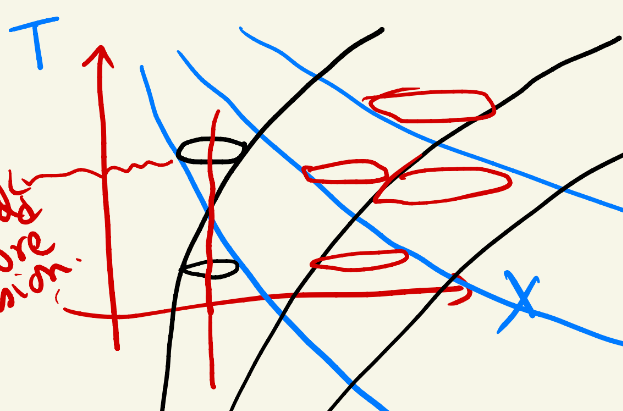
\includegraphics[width=0.5\linewidth]{t=lnx.png}

\end{solution}
\newpage
Now if the metric is not a minkowski metric the We have to take the differentiation of the Metric therm also i.e. of $g_{ij}$
Giving us the \textbf{Geodesic Equation}
\[ \frac{d^2x^{\beta}}{d\tau^2} + \sum_{\nu,\mu}\varGamma^\beta_{\mu\nu} \frac{dx^{\mu}}{d\tau}\frac{dx^{\nu}}{d\tau} = 0   \]
Where $\varGamma^\beta_{\mu\nu} = \frac{1}{2}g^{\beta\mu} [\partial_\sigma g_{\mu\nu}+\partial_\nu g_{\mu\sigma}-\partial_\mu g_{\sigma\nu} ]$ and $\partial_\mu x_\nu = \frac{\partial x_\nu}{\partial \mu}$

\section{Covariant Derivative}
Covariant derivative acts on $(k,l)$ Tensors field and convert to $(k,l+1)$ tensor field.
It is denoted by $\bigtriangledown$
\\ 
Covariant derivative on a vector field:
$\nabla V$ is a $rank (1,1)$ tensor where V is a vector.
\[ \nabla_\mu V^\nu = \partial_\mu V^\nu + C_{\mu\lambda }^\nu V^\lambda  \] where $C_{\mu\lambda }$ is a linear transformation.
\begin{exercise}
    The $C_{\mu\lambda }^\nu$ is not a tensor
\end{exercise}
\begin{solution}
\[ \nabla_{\mu'} V^{\nu'} = \partial_{\mu'} V^{\nu'} + C_{\mu'\lambda' }^{\nu'} V^{\lambda'}  \]
also \[ \nabla_{\mu'} V^{\nu'} = \frac{dx^\mu}{dx^{\mu'}}\frac{dx^{\nu'}}{dx^\nu}\nabla_\mu V^\nu and \nabla_\mu V^\nu = \partial_\mu V^\nu + C_{\mu\lambda }^\nu V^\lambda  \]

Thus using the above 2 results we get that \[ C_{\mu'\lambda' }^{\nu'} = \frac{dx^\mu}{dx^{\mu'}}\frac{dx^\lambda}{dx^{\lambda'}}\frac{dx^{\nu'}}{dx^\nu} C_{\mu\lambda }^\nu - \frac{dx^\mu}{dx^{\mu'}}\frac{dx^\lambda}{dx^{\lambda'}}\frac{d^2x^{\nu'}}{dx^\mu dx^\lambda} \]
Which is not a tensor transformation law.    
\end{solution}
\\
$C_{\mu\lambda }^\nu$ is called as \textbf{Connection Coefficient}.
\\
\\The Covariant derivative follows the following properties:
\begin{itemize}
    \item Linearity \[ \nabla(T+S) = \nabla T + \nabla S \]
    \item  Product Rule \[\nabla(T\otimes S) = \nabla T \otimes S +T\otimes \nabla S\]
    \item All $\nabla $ operators obeying the above rules follow \[ \nabla_\mu f = \partial_\mu f \]
\end{itemize}
Covariant Derivative of Covector is defined in a similar way as Covariant Derivative of Vectors.
\[\nabla_\mu w_\nu = \partial_\mu w_\nu + \widetilde{C}_{\mu\lambda }^\nu w_\lambda\] 

Now it  is found out that the $\widetilde{C}_{\mu\lambda }^\nu = -C_{\mu\lambda }^\nu$

$C_{\mu\lambda }^\nu$ is not a tensor but $C_{\mu\lambda }^\nu - C_{\lambda\mu }^\nu$ is a $rank (1,2)$ tensor called \textbf{Torsion Tensor}.
\\
We demand some more conditions on the Covariant Derivative as follows:
\begin{itemize}
    \item $C_{\mu\lambda }^\nu = C_{\lambda\mu }^\nu$
    \item $\nabla_\rho g_{\mu\nu} = 0 $ i.e. \[ \nabla_\rho g_{\mu\nu} = \partial_\rho g_{\mu\nu} - C_{\rho\mu }^\lambda g_{\lambda\nu} -C_{\rho \nu }^\lambda g_{\mu\lambda} =0 \]
\end{itemize}


These conditions give a unique Connection known as Levi-Civita connection also known as Christoffel symbol discussed earlier 
$\varGamma^\beta_{\mu\nu} = \frac{1}{2}g^{\beta\mu} [\partial_\sigma g_{\mu\nu}+\partial_\nu g_{\mu\sigma}-\partial_\mu g_{\sigma\nu} ]$ and $\partial_\mu x_\nu = \frac{\partial x_\nu}{\partial \mu}$











\end{document}
